\documentclass[journal]{IEEEtran}
\usepackage{graphicx,booktabs,xcolor,amsmath,amssymb,url,cite,multirow}
\usepackage{algorithm,algpseudocode}
\usepackage{tikz}
\usetikzlibrary{arrows.meta}
\graphicspath{{../../results/figures/}}
\providecommand{\tbd}{\textcolor{red}{\textbf{TBD}}}
\newcommand{\dmMAE}{9.2}
\newcommand{\dmR}{0.60}
\newcommand{\dmRtwo}{0.35}
\newcommand{\dmN}{200}
\newcommand{\hcMAE}{7.4}
\newcommand{\hcR}{0.53}
\newcommand{\hcRtwo}{-1.9}
\newcommand{\biasA}{0.88}
\newcommand{\bagHC}{0.0}
\newcommand{\bagHCsd}{8.7}
\newcommand{\bagAD}{-11.2}
\newcommand{\bagADsd}{14.2}
\newcommand{\bagFTD}{-2.2}
\newcommand{\bagFTDsd}{17.8}
\newcommand{\bagD}{-0.93}
\newcommand{\bagWelchP}{p < 0.001}
\newcommand{\bagMwuP}{p < 0.001}
\newcommand{\bagWelchT}{-3.90}
\newcommand{\bagDci}{[$-1.52$, $-0.46$]}
\newcommand{\bagDiffCI}{[$-16.9$, $-5.6$]}
\newcommand{\bagAUCci}{[$0.56$, $0.82$]}
\newcommand{\bagPermP}{p = 0.002}
\newcommand{\bagAUC}{0.70}
\newcommand{\bagAcc}{66\%}
\newcommand{\bagPrec}{68\%}
\newcommand{\bagRec}{72\%}
\newcommand{\bagSpec}{59\%}
\newcommand{\bagFone}{0.70}
\newcommand{\bagThr}{-2.6}
\newcommand{\ftdHCd}{-0.17}
\newcommand{\ftdHCp}{p = 0.87}
\newcommand{\adFTDd}{-0.57}
\newcommand{\adFTDp}{p = 0.04}
\newcommand{\mmseRho}{-0.08}
\newcommand{\mmseP}{p = 0.62}
\newcommand{\nStable}{12}
\newcommand{\nStableYounger}{12}
\newcommand{\nConfigs}{36}
\newcommand{\stableDlo}{-0.99}
\newcommand{\stableDhi}{-0.26}
\newcommand{\icaD}{-0.70}
\newcommand{\icaP}{p = 0.02}
\newcommand{\repD}{-0.83}
\newcommand{\repAUC}{0.71}
\newcommand{\repPermP}{p = 0.003}
\newcommand{\repHCMAE}{12.6}
\newcommand{\repADFTDp}{p = 0.002}
\newcommand{\repDmMAE}{8.4}
\newcommand{\repDmR}{0.71}
\newcommand{\cnnAUC}{0.89}
\newcommand{\cnnAUCsd}{0.03}
\newcommand{\cnnAcc}{82\%}
\newcommand{\cnnAccsd}{2\%}
\newcommand{\cnnBalAcc}{82\%}
\newcommand{\cnnBalAccsd}{3\%}
\newcommand{\cnnPrec}{84\%}
\newcommand{\cnnPrecsd}{4\%}
\newcommand{\cnnRec}{83\%}
\newcommand{\cnnRecsd}{0\%}
\newcommand{\cnnSpec}{80\%}
\newcommand{\cnnSpecsd}{5\%}
\newcommand{\cnnFone}{0.84}
\newcommand{\cnnFonesd}{0.02}
\newcommand{\cnnAUClo}{0.86}
\newcommand{\cnnAUChi}{0.90}
\newcommand{\cnnPrimAUC}{0.86}
\newcommand{\cnnPrimAUCci}{[$0.76$, $0.94$]}
\newcommand{\cnnPrimAcc}{80\%}
\newcommand{\cnnPrimAccci}{[69, 89]\%}
\newcommand{\cnnPermP}{\tbd{}}
\newcommand{\cnnPermN}{\tbd{}}
\newcommand{\cnnPermNull}{\tbd{}}
\newcommand{\cnnPermNullMax}{\tbd{}}
\newcommand{\cnnFinalEpochs}{3}
\newcommand{\bestModel}{EEGNet (raw EEG)}
\newcommand{\bestModelAUC}{0.88}
\newcommand{\modelAUClo}{0.84}
\newcommand{\modelAUChi}{0.88}
\newcommand{\minDiffP}{0.63}
\newcommand{\combAUC}{0.87}
\newcommand{\combAcc}{78\%}
\newcommand{\combCnnAUC}{0.86}
\newcommand{\combBagAUC}{0.73}
\newcommand{\combDiff}{0.01}
\newcommand{\combDiffCI}{[$-0.06$, $0.08$]}
\newcommand{\combP}{p = 0.74}
\newcommand{\ablFull}{0.89}
\newcommand{\ablSlow}{0.85}
\newcommand{\ablFast}{0.87}
\newcommand{\ablNoTime}{0.84}
\newcommand{\ablEight}{0.85}
\newcommand{\ablSixty}{0.88}
\newcommand{\ablMaxDrop}{0.05}
\newcommand{\mcCNNBalAcc}{63\%}
\newcommand{\mcCNNMacroF}{0.63}
\newcommand{\mcCNNMacroAUC}{0.78}
\newcommand{\mcCNNAcc}{65\%}
\newcommand{\mcRFBalAcc}{56\%}
\newcommand{\mcRFMacroF}{0.55}
\newcommand{\mcRFMacroAUC}{0.72}
\newcommand{\mcRFAcc}{59\%}
\newcommand{\mcRecHC}{76\%}
\newcommand{\mcRecAD}{69\%}
\newcommand{\mcRecFTD}{45\%}
\newcommand{\mcFTDasAD}{10}
\newcommand{\mcNFTD}{22}
\newcommand{\gcOOFADdelta}{0.81}
\newcommand{\gcOOFADtheta}{1.29}
\newcommand{\gcOOFADalpha}{1.27}
\newcommand{\gcOOFADbeta}{1.09}
\newcommand{\gcOOFADgamma}{0.64}
\newcommand{\gcOOFHCdelta}{0.65}
\newcommand{\gcOOFHCtheta}{0.96}
\newcommand{\gcOOFHCalpha}{1.35}
\newcommand{\gcOOFHCbeta}{1.47}
\newcommand{\gcOOFHCgamma}{0.94}
\newcommand{\gcFINALADdelta}{0.83}
\newcommand{\gcFINALADtheta}{1.29}
\newcommand{\gcFINALADalpha}{1.39}
\newcommand{\gcFINALADbeta}{1.07}
\newcommand{\gcFINALADgamma}{0.40}
\newcommand{\gcFINALHCdelta}{0.58}
\newcommand{\gcFINALHCtheta}{1.12}
\newcommand{\gcFINALHCalpha}{1.37}
\newcommand{\gcFINALHCbeta}{1.40}
\newcommand{\gcFINALHCgamma}{1.02}
\newcommand{\gcTopChAD}{F8, T6, T3, P4}
\newcommand{\nDortmund}{200}
\newcommand{\nTarget}{87}
\newcommand{\nAD}{36}
\newcommand{\nHC}{29}
\newcommand{\nFTD}{22}

\makeatletter\newcommand{\tableinput}[1]{\@@input ../generated/#1 }\makeatother

\begin{document}

\title{When Alzheimer's EEG Does Not Look Old:\\ A Normative Brain-Age Deviation and Explainable Scalogram CNNs for Alzheimer's Disease Detection}

\author{Aayush~Soni, Aamal~Moshin~Magdum, Afreen~Anz, and~Aparna~Sankar%
\thanks{The authors are with the Department of Computer Science and Engineering, B.\,M.\,S. College of Engineering, Bengaluru, India.}}

\markboth{Draft for internal review}{Soni \MakeLowercase{\textit{et al.}}: When Alzheimer's EEG Does Not Look Old}

\maketitle

% =====================================================================
\begin{abstract}
\emph{Objective:} Resting-state electroencephalography (EEG) is an inexpensive, scalable candidate for Alzheimer's disease (AD) screening. Brain-age models, trained on healthy people and read through the brain-age gap (BAG), are widely assumed to show ``accelerated aging'' in neurodegeneration. We tested this assumption for resting-state EEG in AD and developed an explainable deep-learning classifier, both under strictly subject-independent evaluation.
\emph{Methods:} One harmonized preprocessing pipeline fed two modules. (i) A spectral brain-age model was trained on \dmN{} healthy adults aged 20--70 years (Dortmund Vital Study) and transferred to a clinical cohort of \nAD{} AD, \nHC{} healthy-control (HC) and \nFTD{} frontotemporal-dementia (FTD) subjects (OpenNeuro ds004504); patients were never used for training. (ii) A compact convolutional neural network (CNN) was trained on Morlet continuous-wavelet-transform (CWT) scalograms, explained with Grad-CAM, and compared with four baselines on identical subject folds. Robustness was assessed across \nConfigs{} model configurations, ICA-cleaned data, a \repNok{}-subject replication, a 20--80-year normative training set and an external healthy cohort (MPI-LEMON).
\emph{Results:} The bias-corrected BAG was strongly \emph{negative} in AD ($\bagAD{}\pm\bagADsd{}$ vs. $\bagHC{}\pm\bagHCsd{}$ years; Cohen's $d=\bagD{}$, 95\% CI \bagDci{}). The effect was absent in FTD ($d=\ftdHCd{}$), negative in all \nStable{} numerically stable configurations, and not shown by healthy older adults from an independent site (AD vs.\ external HC, $d=\lemADd{}$). Feature analysis showed that slow-wave power and the aperiodic exponent fall and beta power rises with healthy aging, whereas AD shows the opposite. The CNN reached AUC \cnnAUC{} and accuracy \cnnAcc{} (three seeds), statistically indistinguishable from spectral baselines and EEGNet. Adding BAG did not improve it ($\Delta$AUC $=\combDiff{}$, \combP{}). Grad-CAM emphasized theta and alpha activity, consistently in- and out-of-fold.
\emph{Conclusion:} In resting-state EEG, AD does not resemble an older healthy brain. It departs from the normative aging trajectory. EEG brain age in AD should therefore be read as a normative-deviation score rather than as accelerated aging.
\end{abstract}

\begin{IEEEkeywords}
Alzheimer's disease, electroencephalography, brain age, normative modeling, continuous wavelet transform, convolutional neural network, explainable AI, Grad-CAM
\end{IEEEkeywords}

% =====================================================================
\section{Introduction}
\IEEEPARstart{A}{lzheimer's} disease (AD) is the leading cause of dementia. Its diagnosis relies on clinical assessment, neuropsychological testing and, increasingly, MRI, PET or fluid biomarkers. These tools are expensive or invasive and scarce in many health systems, so inexpensive, scalable screening remains an unmet need. Resting-state electroencephalography (EEG) is non-invasive, portable and widely available. AD alters it in a characteristic way, often summarized as ``slowing'': delta and theta activity increase, alpha and beta activity decrease, and the dominant alpha rhythm moves to lower frequencies~\cite{jeong2004,babiloni2020}.

Two computational strategies exploit these changes. \emph{Discriminative classifiers} learn to separate patients from controls. They range from band-power features with classical machine learning to deep networks on raw signals or time--frequency images~\cite{craik2019,roy2019}. They can be accurate, but their decisions are often hard to interpret, and their reported accuracy is inflated when evaluation is not subject-independent~\cite{roy2019,varoquaux2018}. \emph{Brain-age models} take a normative route. A regressor is trained only on healthy people to predict chronological age, and the brain-age gap (BAG, predicted minus chronological age) of a new person is read as a marker of accelerated or delayed aging~\cite{cole2017,franke2019}. Brain age is intuitive and continuous, and it does not require patient data for training. However, it rests on a strong assumption: disease moves the brain \emph{along} the healthy-aging trajectory. This assumption has been supported for structural MRI and for sleep EEG in dementia~\cite{sun2019}. It has rarely been tested for resting-state EEG in clinically diagnosed AD with a model that never sees patients.

We developed and rigorously evaluated both strategies on public data. Our contributions are:
\begin{enumerate}
\item \emph{A normative EEG brain-age module} that is trained only on healthy adults and transferred to a clinical cohort without using patients for training, harmonization or model selection.
\item \emph{A robust negative finding.} In AD the EEG brain-age gap is strongly \emph{negative}, specific to AD versus FTD, and stable across configurations, preprocessing choices and training sets, and not reproduced by healthy older adults from an independent site. Feature-level analysis explains it by spectral changes that run in opposite directions in aging and AD.
\item \emph{An explainable CWT-scalogram CNN}, compared with four baselines on identical subject folds, with ablations, a three-class (HC/AD/FTD) extension, and Grad-CAM evaluated both in- and out-of-fold.
\item \emph{An honest assessment of combining the modules} (BAG adds interpretability, not accuracy), and an open implementation that includes an application producing a per-person report.
\end{enumerate}

% =====================================================================
\section{Related Work}
\subsection{EEG signatures of Alzheimer's disease}
Decades of quantitative EEG research report a consistent AD profile: increased delta and theta power, reduced alpha and beta power, a lower alpha peak frequency and altered functional connectivity~\cite{jeong2004,babiloni2020}. Importantly, the electrophysiology of AD is not simply an exaggeration of normal aging. Babiloni et al.\ distinguish the pathological slowing of AD from the more modest spectral changes of healthy aging~\cite{babiloni2020}. This distinction motivates our test of the brain-age assumption.

\subsection{Machine and deep learning for EEG-based diagnosis}
Classical pipelines extract band powers, spectral ratios or complexity measures and apply support vector machines, random forests or regularized linear models. Deep learning learns representations directly from raw signals or from time--frequency images such as spectrograms and wavelet scalograms~\cite{craik2019,roy2019}. EEGNet~\cite{eegnet} is a widely used compact architecture designed for small EEG datasets. Systematic reviews caution that many reported accuracies come from epoch-level or subject-dependent splits, in which data from the same person appear in training and test, and from small samples with wide error bars~\cite{roy2019,varoquaux2018}. We therefore use subject-level splits throughout, compare against baselines on identical folds, and report confidence intervals and permutation tests.

\subsection{Brain age and the brain-age gap}
Brain-age prediction is an established biomarker framework in neuroimaging~\cite{cole2017,franke2019}. Because regression to the mean biases raw gaps, predictions must be bias-corrected~\cite{delange2020}. EEG-based brain age has been estimated from resting-state recordings with classical and deep models~\cite{alzoubi2018,engemann2022}. Sleep-EEG brain age was elevated in people with dementia~\cite{sun2019}, which supports the accelerated-aging view. Normative modeling generalizes brain age by describing how each measure varies in a healthy reference population and quantifying individual deviations from it. Our results suggest that this deviation view, rather than the accelerated-aging view, fits resting-state EEG in AD.

\subsection{Explainability and multi-site harmonization}
Gradient-weighted class activation mapping (Grad-CAM)~\cite{gradcam} produces class-specific importance maps from the last convolutional layer of a CNN. On scalograms these maps can be read as frequency-by-time importance and checked against known physiology. Pooling data across sites requires harmonization. ComBat~\cite{johnson2007} removes additive and multiplicative site effects with empirical Bayes shrinkage while protecting biological covariates, and has been adopted widely in neuroimaging~\cite{fortin2018}.

% =====================================================================
\section{Proposed Methodology}
Fig.~\ref{fig:pipeline} shows the system. A single harmonized preprocessing stage feeds a brain-age module (teal) and a CNN classifier (orange). Both outputs are reported per subject and can be combined.

\begin{figure}[t]
\centering
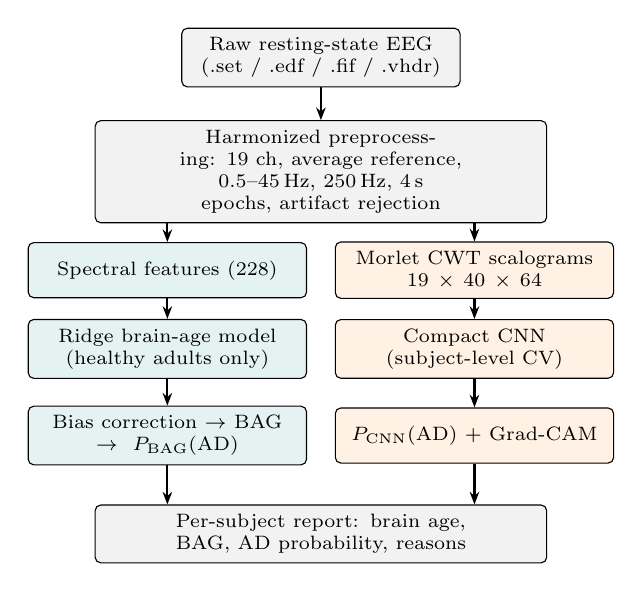
\begin{tikzpicture}[every node/.style={font=\scriptsize},
  box/.style={draw, rounded corners=2pt, align=center, minimum height=7mm, text width=3.3cm, fill=#1!10},
  box/.default=gray, ar/.style={-{Stealth[length=1.6mm]}, thick}]
\node[box=gray] (raw) at (0,0.45) {Raw resting-state EEG (.set / .edf / .fif / .vhdr)};
\node[box=gray, text width=5.5cm] (pre) at (0,-1.0) {Harmonized preprocessing: 19 ch, average reference,\\0.5--45\,Hz, 250\,Hz, 4\,s epochs, artifact rejection};
\node[box=teal] (feat) at (-1.95,-2.25) {Spectral features (228)};
\node[box=teal] (ba) at (-1.95,-3.25) {Ridge brain-age model\\(healthy adults only)};
\node[box=teal] (bag) at (-1.95,-4.35) {Bias correction $\rightarrow$ BAG\\$\rightarrow P_\mathrm{BAG}(\mathrm{AD})$};
\node[box=orange] (cwt) at (1.95,-2.25) {Morlet CWT scalograms\\$19\times40\times64$};
\node[box=orange] (cnn) at (1.95,-3.25) {Compact CNN\\(subject-level CV)};
\node[box=orange] (gc) at (1.95,-4.35) {$P_\mathrm{CNN}(\mathrm{AD})$ + Grad-CAM};
\node[box=gray, text width=5.5cm] (rep) at (0,-5.6) {Per-subject report: brain age, BAG, AD probability, reasons};
\draw[ar] (raw) -- (pre); \draw[ar] (pre.south) ++(-1.95,0) -- (feat); \draw[ar] (pre.south) ++(1.95,0) -- (cwt);
\draw[ar] (feat) -- (ba); \draw[ar] (ba) -- (bag); \draw[ar] (cwt) -- (cnn); \draw[ar] (cnn) -- (gc);
\draw[ar] (bag.south) -- (bag.south |- rep.north); \draw[ar] (gc.south) -- (gc.south |- rep.north);
\end{tikzpicture}
\caption{Proposed pipeline. Teal: normative brain-age module. Orange: explainable CNN classifier.}
\label{fig:pipeline}
\end{figure}

\subsection{Harmonized preprocessing}
Every recording, whether training, test or uploaded, passes through one function implemented with MNE-Python~\cite{mne}. The function: (1) maps 10--10 channel names to 10--20 (T7/T8/P7/P8$\rightarrow$T3/T4/T5/T6) and selects 19 channels in a fixed order (Fp1, Fp2, F7, F3, Fz, F4, F8, T3, C3, Cz, C4, T4, T5, P3, Pz, P4, T6, O1, O2); (2) re-references to their average; (3) band-pass filters at 0.5--45\,Hz (zero-phase FIR); (4) resamples to 250\,Hz; (5) cuts 4\,s epochs with 2\,s overlap; and (6) rejects epochs whose peak-to-peak amplitude on any channel exceeds 150\,$\mu$V or falls below 1\,$\mu$V. Recordings shorter than 30\,s or with fewer than 10 clean epochs are rejected with an explanatory message. ICA is deliberately not used, so that the same deterministic pipeline applies at deployment. Its effect is tested with ICA-cleaned data. For recordings that alternate eyes-open and eyes-closed blocks (LEMON), only eyes-closed blocks are kept and joined, and filtering and epoching never cross the joins.

\subsection{Spectral features}
For each subject, Welch power spectra (4\,s Hann window, 0.25\,Hz resolution) are averaged over clean epochs. Per channel we compute the following:
\begin{itemize}
\item log absolute power $\log_{10}\!\int_{b} P(f)\,df$ in the delta (1--4\,Hz), theta (4--8), alpha (8--13) and beta (13--30\,Hz) bands;
\item relative power, the band power divided by power over 1--45\,Hz;
\item the alpha peak frequency, $\arg\max_{f\in[7,13]}P(f)$;
\item the log theta/alpha ratio;
\item the aperiodic exponent and offset, from a FOOOF fit~\cite{fooof} over 2--40\,Hz.
\end{itemize}
This yields 228 features per subject (12 per channel), plus 60 regional averages used in one model variant.

\subsection{Brain-age module}
\emph{Model.} Ridge regression on standardized features predicts chronological age. The regularization strength is tuned by inner 5-fold cross-validation over $\alpha\in[10^{-2},10^{5}]$. During development we also evaluated a sign-constrained ridge, in which each weight must follow its feature's marginal age direction, and gradient boosting. Both appear in the robustness analysis.

\emph{Transfer and leakage control.} The clinical cohort spans a narrow age range and was recorded with different equipment from the healthy cohort. We therefore compared four strategies: (a) healthy cohort only; (b) healthy cohort plus clinical HC, each HC predicted out-of-fold by leave-one-HC-out; (c) ComBat harmonization~\cite{johnson2007,fortin2018}, with age protected and fitted on healthy subjects only; and (d) (b) and (c) combined. AD and FTD subjects never enter training, harmonization or selection. The final configuration was chosen by a rule fixed in advance that does not look at patients: features and model by healthy-cohort CV error, then strategy by out-of-fold clinical-HC error.

\emph{Bias correction and BAG.} On out-of-fold HC predictions we fit $\hat{y}=a\,y+b$ and define corrected age $\tilde{y}=(\hat{y}-b)/a$ and $\mathrm{BAG}=\tilde{y}-y$~\cite{delange2020}. The parameters are fitted on HC only. A logistic model maps BAG to $P_\mathrm{BAG}(\mathrm{AD})$. Its cross-validation refits the bias correction inside every fold.

\subsection{CWT-scalogram CNN}
\emph{Input.} Each clean epoch is transformed with complex Morlet wavelets at 40 log-spaced frequencies from 1 to 40\,Hz ($n_\mathrm{cycles}=\mathrm{clip}(f/2,2,10)$). Log power is pooled into 64 time bins, which gives a $19\times40\times64$ tensor with channels as input feature maps. Up to 150 evenly spaced epochs per subject are used.

\emph{Architecture.} Three blocks of $3\times3$ convolution, batch normalization and ReLU (16, 32 and 32 filters; the first two are followed by $2\times2$ max-pooling), then global average pooling, dropout 0.5 and a linear output: about 17k parameters in total. The network is deliberately small because the cohort is small.

\emph{Training.} We use Adam (learning rate $10^{-3}$, weight decay $10^{-3}$, batch size 128) and binary cross-entropy weighted by class frequency. Inputs are standardized per channel and frequency using training subjects only. Early stopping monitors the loss of validation \emph{subjects} (15\% of the training side; patience 6; at most 40 epochs). A subject's $P_\mathrm{CNN}(\mathrm{AD})$ is the mean of its epoch probabilities.

\emph{Explainability.} For the last convolutional activations $A^k$ and logit $y^c$, Grad-CAM computes $L^c=\mathrm{ReLU}\big(\sum_k w_k^c A^k\big)$ with $w_k^c=\frac{1}{Z}\sum_{i,j}\partial y^c/\partial A^k_{ij}$~\cite{gradcam}. The map is bilinearly upsampled to the $40\times64$ grid. Band importance is the mean map value within a band divided by the mean over all frequencies, so 1.0 means average importance. This removes the bias from wider log-spaced bands. Channel importance uses gradient$\times$input summed per channel.

\subsection{Baselines, combination and evaluation protocol}
On the CNN's \emph{identical} subject folds we evaluated: logistic regression, RBF-SVM and random forest on the 228 spectral features, with hyper-parameters tuned by inner 5-fold CV on training subjects; and EEGNet-8,2~\cite{eegnet} on raw epochs, using the same training loop and early stopping as the CNN. CNN and BAG were combined by stacking: logistic regression on $[\mathrm{logit}\,P_\mathrm{CNN},\mathrm{BAG}]$, evaluated with 20$\times$ repeated stratified 5-fold CV.

All classification metrics are subject-level and out-of-fold. The CNN was run with three seeds; each seed changes both the fold assignment and the initialization. We report AUC, accuracy, balanced accuracy, precision, recall (sensitivity), specificity and F1. Confidence intervals use 2000 subject-level bootstrap resamples, stratified by class. The significance of cross-validated AUC is assessed by permutation tests that shuffle labels across subjects and re-run the \emph{entire} cross-validation~\cite{ojala2010}. AUC differences between models use a paired bootstrap. Group differences in BAG use Welch's $t$-test, the Mann--Whitney $U$ test and Cohen's $d$ with bootstrap CIs.

% =====================================================================
\section{Algorithms}

\begin{algorithm}[t]
\caption{Harmonized preprocessing}
\label{alg:pre}
\begin{algorithmic}[1]
\Require EEG recording $R$; channel list $\mathcal{C}$ (19 channels, 10--20)
\Ensure clean epochs $X \in \mathbb{R}^{n\times19\times1000}$
\State map 10--10 names (T7, T8, P7, P8) to 10--20 (T3, T4, T5, T6)
\If{a channel of $\mathcal{C}$ is missing or duration $< 30$\,s} \State \textbf{reject} with an explanatory message \EndIf
\State optionally keep only eyes-closed blocks (alternating protocols)
\State select $\mathcal{C}$ in fixed order; re-reference to their average
\State band-pass 0.5--45\,Hz (zero-phase FIR); resample to 250\,Hz
\State cut 4\,s epochs with 2\,s overlap (never across block boundaries)
\State keep epoch $e$ iff $1\,\mu\mathrm{V} < \mathrm{ptp}_c(e) < 150\,\mu\mathrm{V}$ for every channel $c$
\If{fewer than 10 epochs remain} \State \textbf{reject} \EndIf
\State \Return $X$ (cached by configuration hash)
\end{algorithmic}
\end{algorithm}

\begin{algorithm}[t]
\caption{Normative brain-age training, transfer and BAG}
\label{alg:ba}
\begin{algorithmic}[1]
\Require healthy cohort $D_H$; clinical HC $T_C$; patients $T_P$ (AD, FTD)
\Ensure BAG for every clinical subject
\For{each $s \in T_C$} \Comment{leave-one-HC-out}
  \State fit ridge (inner-CV $\alpha$) on $D_H \cup T_C\setminus\{s\}$
  \State $\hat{y}_s \gets$ predicted age of $s$
\EndFor
\State fit ridge on $D_H \cup T_C$; $\hat{y}_p \gets$ prediction for each $p \in T_P$
\State fit $\hat{y} = a\,y + b$ on $\{(y_s,\hat{y}_s): s\in T_C\}$ \Comment{HC only}
\State $\mathrm{BAG}_i \gets (\hat{y}_i - b)/a - y_i$ for every clinical subject $i$
\State \Return BAG; fit $P(\mathrm{AD}\mid\mathrm{BAG})$ by logistic regression
\end{algorithmic}
\end{algorithm}

\begin{algorithm}[t]
\caption{Subject-level cross-validation of the CNN}
\label{alg:cnn}
\begin{algorithmic}[1]
\Require subjects $S$ with labels; scalograms $Z_s$ ($\le150$ per subject); seed $r$
\Ensure out-of-fold $P(\mathrm{AD})$ for every subject
\State split $S$ into 10 stratified folds $F_1,\dots,F_{10}$ (seed $r$)
\For{$k = 1$ to $10$}
  \State $S_\mathrm{tr} \gets S \setminus F_k$; split into fit (85\%) / validation (15\%) subjects
  \State standardize with mean/SD per channel$\times$frequency of fit subjects
  \State train CNN on fit epochs (Adam, class-weighted BCE)
  \State early-stop on validation-subject loss (patience 6); restore best weights
  \For{each $s \in F_k$} \State $P_s \gets$ mean epoch probability of $s$ \EndFor
\EndFor
\State \Return $\{P_s\}$ \Comment{no subject in both training and test}
\end{algorithmic}
\end{algorithm}

\begin{algorithm}[t]
\caption{Inference and report for a new subject}
\label{alg:inf}
\begin{algorithmic}[1]
\Require EEG file, chronological age $y$
\State $X \gets$ Algorithm~\ref{alg:pre}(file)
\State $\hat{y} \gets$ ridge(features($X$)); $\mathrm{BAG} \gets (\hat{y}-b)/a - y$
\State $P_\mathrm{CNN} \gets$ mean CNN probability over scalograms of $X$
\State compute Grad-CAM band importance toward the predicted class
\State compare alpha peak, band shares and BAG with HC/AD reference values
\State \Return brain age, BAG, $P_\mathrm{CNN}$, $P_\mathrm{BAG}$, combined $P$, reasons
\end{algorithmic}
\end{algorithm}

Algorithms~\ref{alg:pre}--\ref{alg:inf} formalize the pipeline. Two guarantees matter most. Algorithm~\ref{alg:ba} ensures that no patient influences the age model or its bias correction. Algorithm~\ref{alg:cnn} ensures that normalization, early stopping and testing never share subjects. Inference (Algorithm~\ref{alg:inf}) takes about 10\,s per recording on a laptop CPU.

% =====================================================================
\section{Dataset}
Table~\ref{tab:cohorts} summarizes the cohorts. All are public and de-identified.

\begin{table}[t]
\centering
\caption{Cohorts after preprocessing}
\label{tab:cohorts}
\scriptsize\setlength{\tabcolsep}{2.5pt}
\begin{tabular}{lcccc}
\toprule
Cohort & $n$ & Age, mean $\pm$ SD (range) & Female & MMSE \\
\midrule
\tableinput{table_cohorts.tex}
\bottomrule
\end{tabular}
\end{table}

\emph{Clinical cohort: OpenNeuro ds004504}~\cite{miltiadous2023}. Routine clinical resting-state, eyes-closed EEG from AD, FTD and HC participants. It was recorded with a 19-electrode 10--20 montage at 500\,Hz, with MMSE scores. One FTD recording failed artifact screening. The dataset authors' ICA-cleaned derivatives were used only for sensitivity analysis. The dataset contains no mild-cognitive-impairment (MCI) participants, so the primary task is AD vs.\ HC and FTD serves as a specificity control.

\emph{Healthy aging cohort: OpenNeuro ds005385, Dortmund Vital Study}~\cite{gajewski2022}. 64-channel EEG at 1000\,Hz from healthy working-age adults (20--70 years). We used baseline-session, eyes-closed, pre-task recordings and excluded recordings flagged as possibly discontinuous. The main analysis used an age-stratified sample weighted toward older ages (25/25/35/50/65 per decade). A replication used all \repNsel{} eligible subjects (\repNok{} after preprocessing).

\emph{External healthy cohort: MPI-LEMON.} 62-channel EEG at 2500\,Hz from healthy adults, with alternating 1-min eyes-open/eyes-closed blocks. We used the older group (age bins 55--80) and kept only the eyes-closed blocks. Ages are given in 5-year bins, so we used bin midpoints, which adds up to $\pm2.5$ years of label noise. LEMON was never used to train the main model. Its analysis plan was committed to version control before any LEMON data were processed.

\emph{Data quality.} On average about 80\% of epochs were retained for clinical subjects and 90\% for the healthy cohort. Median peak-to-peak amplitudes were similar across cohorts, which confirms consistent units and scaling.

% =====================================================================
\section{Results}
\subsection{Brain age: AD departs from the healthy-aging trajectory}
On the healthy cohort the selected model (ridge, all features, strategy~(b)) achieved MAE \dmMAE{} years ($r=\dmR{}$, $R^2=\dmRtwo{}$) in 10-fold CV. On clinical HC the out-of-fold MAE was \hcMAE{} years ($r=\hcR{}$; bias slope $a=\biasA{}$). The out-of-fold $R^2$ was $\hcRtwo{}$, which is expected for an HC age range of only 57--78 years: any error larger than the 5.4-year SD of age yields a negative $R^2$. We therefore do not use $R^2$ as the success criterion.

The bias-corrected BAG was $\bagHC{}\pm\bagHCsd{}$ years in HC, $\bagAD{}\pm\bagADsd{}$ in AD and $\bagFTD{}\pm\bagFTDsd{}$ in FTD (Fig.~\ref{fig:bag}). AD differed from HC (Welch $t=\bagWelchT{}$, \bagWelchP{}; Mann--Whitney \bagMwuP{}; $d=\bagD{}$, 95\% CI \bagDci{}; mean difference \bagDiffCI{} years). FTD did not differ from HC ($d=\ftdHCd{}$, \ftdHCp{}), and AD differed from FTD ($d=\adFTDd{}$, \adFTDp{}). Within AD, BAG was not associated with MMSE (Spearman $\rho=\mmseRho{}$, \mmseP{}; Fig.~\ref{fig:mmse}).

\begin{figure}[t]
\centering
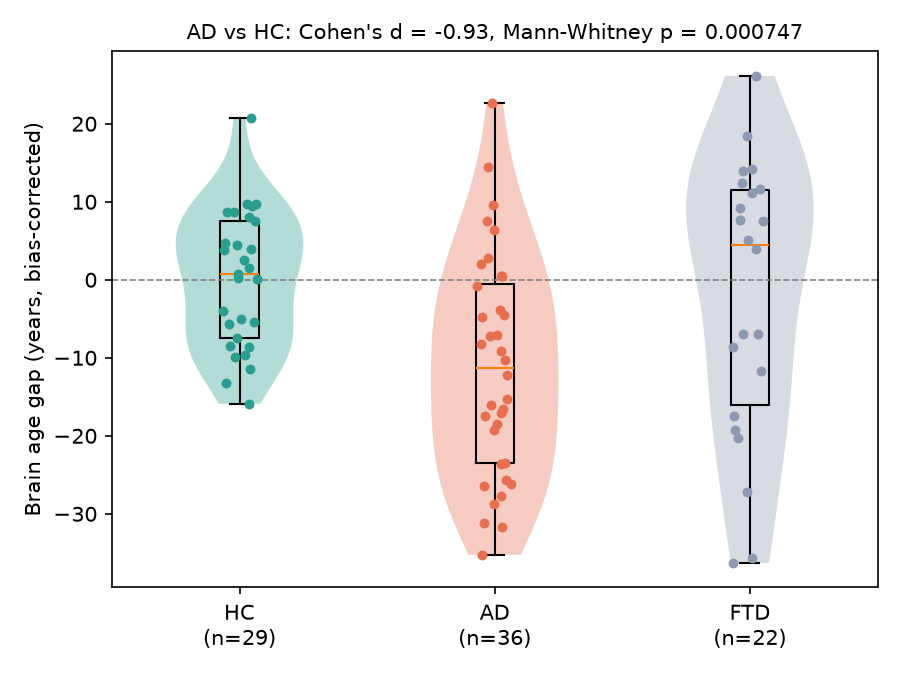
\includegraphics[width=0.92\columnwidth]{bag_by_group.png}
\caption{Bias-corrected brain-age gap by group. HC are out-of-fold; AD and FTD were never used for training.}
\label{fig:bag}
\end{figure}

\emph{Robustness.} The negative AD gap appeared in \nStableYounger{} of \nStable{} numerically stable configurations, defined as bias slope $a>0.3$; smaller slopes make $(\hat{y}-b)/a$ numerically meaningless. Effect sizes ranged from $d=\stableDlo{}$ to $\stableDhi{}$ (Fig.~\ref{fig:robust}). The effect persisted on the dataset authors' ICA-cleaned recordings ($d=\icaD{}$, \icaP{}). It also persisted when the healthy training set was enlarged to \repNok{} subjects ($d=\repD{}$; AUC \repAUC{}; permutation \repPermP{}; AD vs.\ FTD \repADFTDp{}). In that run the healthy-cohort MAE improved to \repDmMAE{} years ($r=\repDmR{}$), but transfer to clinical HC worsened (MAE \repHCMAE{} years), because the clinical HC formed a smaller share of the training set.

\begin{figure}[t]
\centering
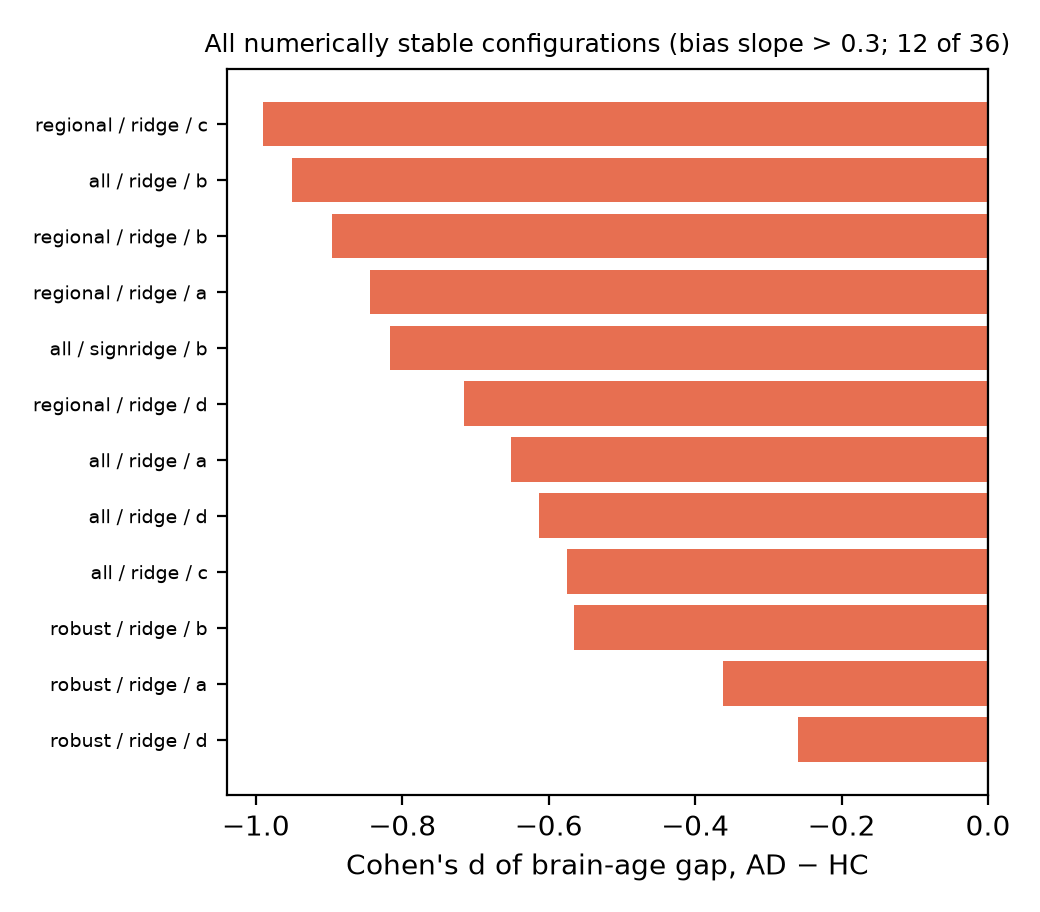
\includegraphics[width=0.95\columnwidth]{bag_robustness.png}
\caption{AD$-$HC effect size of the brain-age gap in every numerically stable configuration (feature set / model / transfer strategy).}
\label{fig:robust}
\end{figure}

\emph{Mechanism.} Table~\ref{tab:dir} and Fig.~\ref{fig:dir} contrast each feature family's correlation with age in healthy adults with its AD--HC effect size. Alpha peak frequency, alpha power and the theta/alpha ratio change in the same direction in aging and AD, so they make AD look ``older''. In contrast, beta power rises with age but falls in AD, and absolute slow-wave power and the aperiodic exponent and offset fall with age but rise in AD. These features make AD look ``younger''. Taken together, AD EEG lies off the normative trajectory and, on balance, ``before'' it.

\begin{table}[t]
\centering
\caption{Healthy-aging direction vs.\ AD effect per feature family}
\label{tab:dir}
\footnotesize\setlength{\tabcolsep}{4pt}
\begin{tabular}{lccc}
\toprule
Feature & $r$ (age, healthy) & $d$ (AD$-$HC) & AD looks \\
\midrule
\tableinput{table_directions.tex}
\bottomrule
\end{tabular}
\end{table}

\begin{figure}[t]
\centering
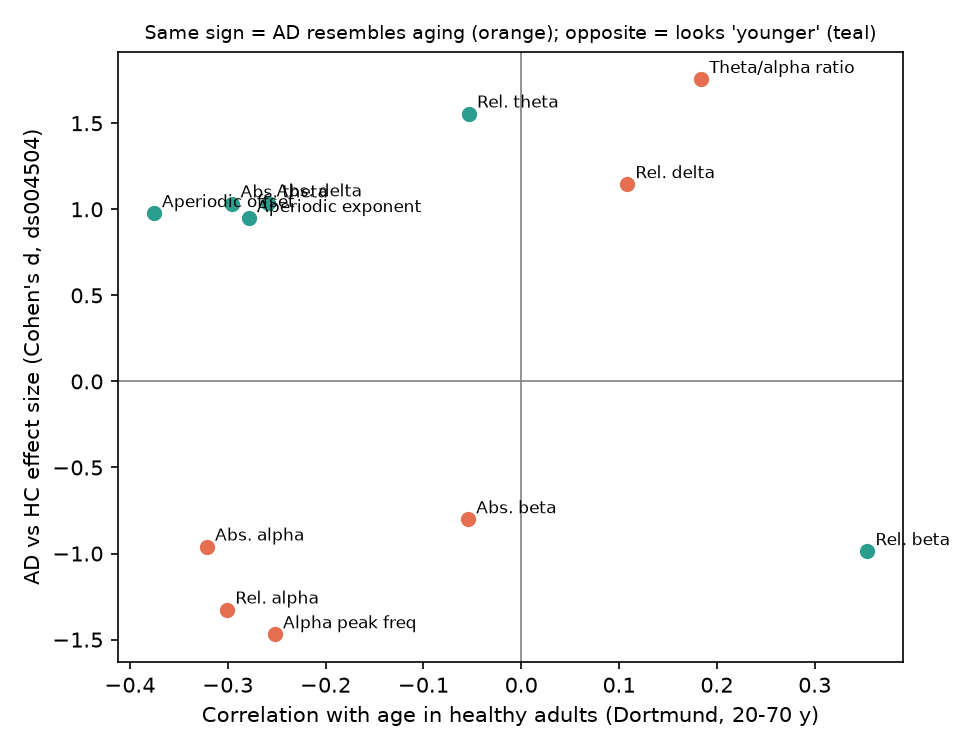
\includegraphics[width=0.92\columnwidth]{feature_directions.png}
\caption{Healthy-aging direction ($x$) vs.\ AD effect ($y$) per feature family. Same sign: AD resembles aging. Opposite sign: AD looks ``younger''.}
\label{fig:dir}
\end{figure}

\begin{figure}[t]
\centering
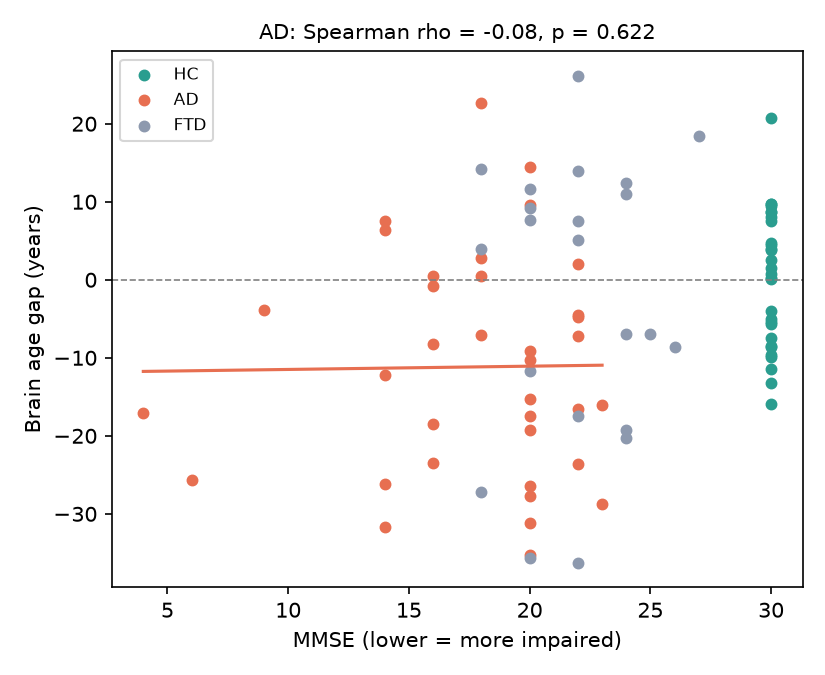
\includegraphics[width=0.8\columnwidth]{bag_vs_mmse.png}
\caption{Brain-age gap vs.\ MMSE. No association within AD.}
\label{fig:mmse}
\end{figure}

\emph{Brain-age gap as a classifier.} Alone, BAG separated AD from HC with AUC \bagAUC{} (95\% CI \bagAUCci{}; permutation \bagPermP{}), accuracy \bagAcc{}, precision \bagPrec{}, recall \bagRec{}, specificity \bagSpec{} and F1 \bagFone{}, using the decision rule BAG $<\bagThr{}$ years.

\subsection{External validation on a third site (MPI-LEMON)}
\emph{Test L1: unchanged model.} Of \lemNavail{} available older LEMON participants, \lemN{} passed preprocessing (one lacked eyes-closed markers). The main model, never trained on LEMON, predicted their age with MAE \lemMAE{} years. Within LEMON the predictions did not track age ($r=\lemR{}$), reflecting the narrow 55--80-year window, 5-year age bins and the model's healthy-cohort error. We compare uncorrected gaps, because the clinical bias correction is site-specific. The mean raw gap was $\rawGapLem{}\pm\rawGapLemsd{}$ years in LEMON HC, $\rawGapHc{}\pm\rawGapHcsd{}$ in clinical HC and $\rawGapAd{}\pm\rawGapAdsd{}$ in AD (Fig.~\ref{fig:lemon}). Healthy older adults from the two independent sites did not differ ($d=\lemHCd{}$, \lemHCp{}), whereas AD differed from the external healthy cohort ($d=\lemADd{}$, \lemADp{}). The strongly negative gap therefore is not reproduced by healthy older adults from an independent laboratory, which argues against a site or age artifact. The moderately negative raw gaps of both healthy groups are consistent with regression toward the mean of a training set that ends at 70 years, which is the bias that the HC-based correction removes.

\emph{Test L2: extended normative training set.} We retrained with healthy cohorts covering 20--80 years ($n=\ltwoN{}$; healthy CV MAE \ltwoMAE{} years) and applied the same patient-blind selection rule. The AD effect was preserved: $d=\ltwoD{}$ (\ltwoP{}; AUC \ltwoAUC{}), negative in \ltwoStableYounger{} of \ltwoStable{} stable configurations, with FTD again unaffected ($d=\ltwoFTDd{}$). Transfer to clinical HC was weaker than in the main model (out-of-fold MAE \ltwoHCMAE{} vs.\ \hcMAE{} years).

\begin{figure}[t]
\centering
\IfFileExists{../../results/figures/external_lemon_l1.png}{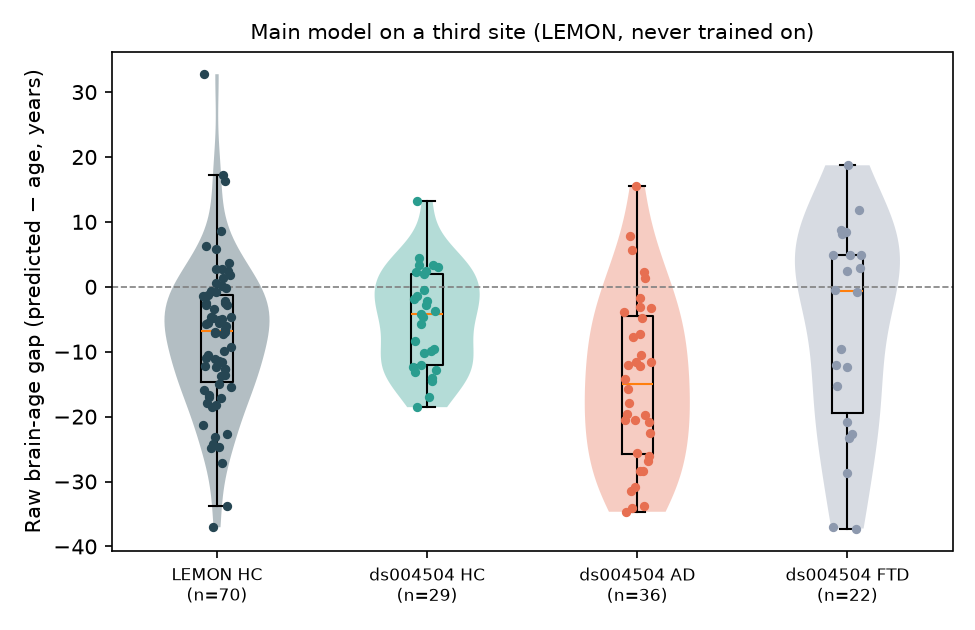
\includegraphics[width=0.95\columnwidth]{external_lemon_l1.png}}{\fbox{\parbox{0.9\columnwidth}{\centering\tbd{} (LEMON analysis running)}}}
\caption{Raw brain-age gaps from the unchanged main model on an external healthy cohort (LEMON) and the clinical cohort.}
\label{fig:lemon}
\end{figure}

\subsection{CNN classification and comparison with baselines}
Table~\ref{tab:seeds} reports the CNN over three seeds. The mean AUC was \cnnAUC{} (range \cnnAUClo{}--\cnnAUChi{}) and the mean accuracy \cnnAcc{}. For the primary seed the AUC was \cnnPrimAUC{} (95\% CI \cnnPrimAUCci{}) and the accuracy \cnnPrimAcc{} (95\% CI \cnnPrimAccci{}). In a permutation test with $N=\cnnPermN{}$ complete re-runs on shuffled labels, the null AUC averaged \cnnPermNull{} (maximum \cnnPermNullMax{}), giving \cnnPermP{} (with $N$ permutations the smallest attainable value is $1/(N+1)$). On identical folds (Table~\ref{tab:base}, Fig.~\ref{fig:roc}), all models performed comparably (AUC \modelAUClo{}--\modelAUChi{}; highest: \bestModel{}, \bestModelAUC{}). No difference from the CNN was significant (all paired-bootstrap $p\geq\minDiffP{}$).

\begin{table}[t]
\centering
\caption{CNN, AD vs.\ HC, subject-level 10-fold CV per seed ($n=65$)}
\label{tab:seeds}
\scriptsize\setlength{\tabcolsep}{2pt}
\begin{tabular}{lcccccc}
\toprule
Seed & AUC & Acc. & Prec. & Rec. & Spec. & F1 \\
\midrule
\tableinput{table_cnn_seeds.tex}
\bottomrule
\end{tabular}
\end{table}

\begin{table*}[t]
\centering
\caption{AD vs.\ HC on identical subject-level 10-fold splits (primary seed, $n=65$). Last column: CNN AUC minus model AUC (paired bootstrap).}
\label{tab:base}
\begin{tabular}{lcccccc}
\toprule
Model & AUC & Acc. (\%) & Recall (\%) & Spec. (\%) & F1 & $\Delta$AUC (CNN$-$model) \\
\midrule
\tableinput{table_baselines.tex}
\bottomrule
\end{tabular}
\end{table*}

\begin{figure}[t]
\centering
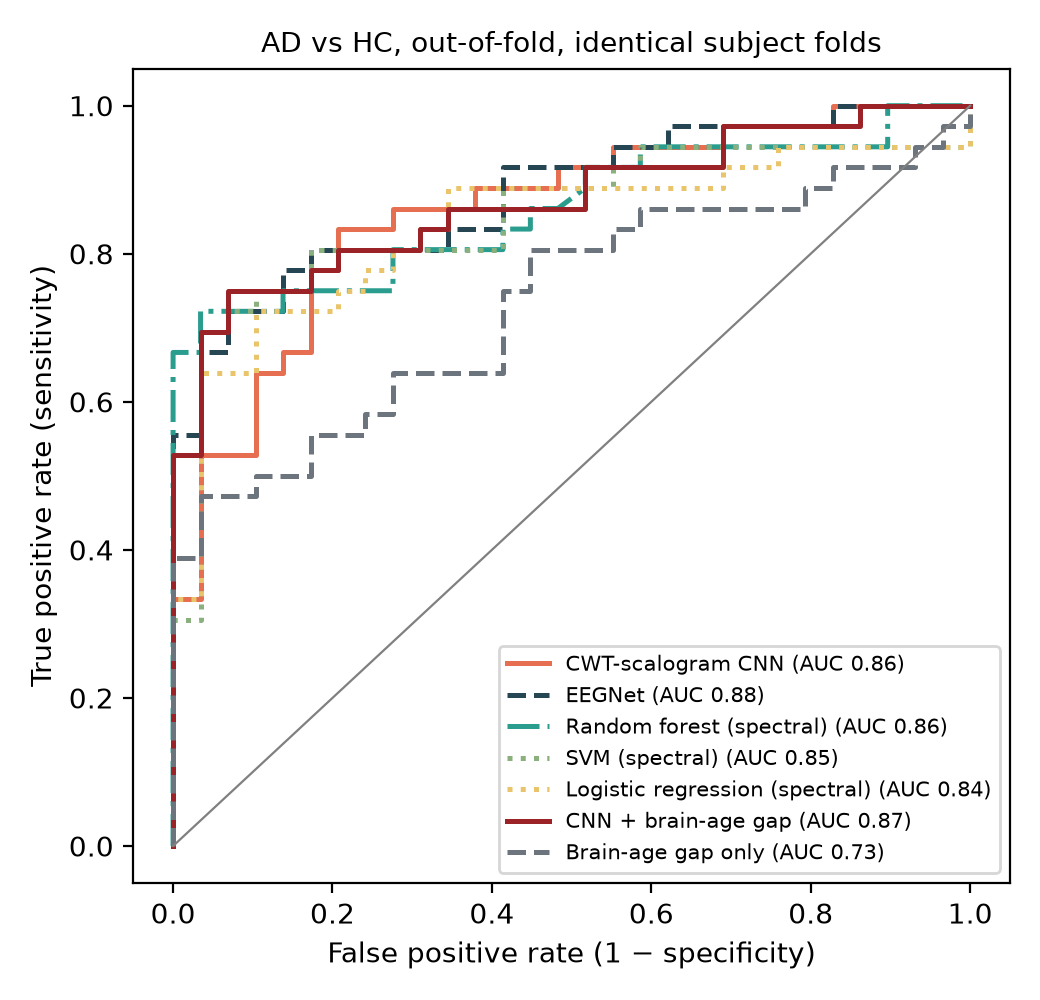
\includegraphics[width=0.85\columnwidth]{roc_all_models.png}
\caption{Out-of-fold ROC curves on identical subject folds.}
\label{fig:roc}
\end{figure}

\subsection{Combining the CNN with the brain-age gap}
Stacking gave AUC \combAUC{} versus \combCnnAUC{} for the CNN alone and \combBagAUC{} for BAG alone ($\Delta=\combDiff{}$, 95\% CI \combDiffCI{}, \combP{}). Both modules draw on the same EEG slowing, so BAG contributes an interpretable continuous score rather than additional accuracy.

\subsection{Ablations}
Each variant in Table~\ref{tab:abl} changes one design choice (three seeds each). No change reduced the mean AUC by more than \ablMaxDrop{}, which is within the seed-to-seed variation. Information was present in both slow (1--8\,Hz, AUC \ablSlow{}) and fast (8--40\,Hz, \ablFast{}) bands, and removing the time axis cost little (\ablNoTime{}). An 8-channel montage (\ablEight{}) and 40\% of the epochs (\ablSixty{}) remained close to the full model (\ablFull{}). This supports low-density, short recordings for screening.

\begin{table}[t]
\centering
\caption{CNN ablations (mean $\pm$ SD over seeds)}
\label{tab:abl}
\footnotesize\setlength{\tabcolsep}{3pt}
\begin{tabular}{lccc}
\toprule
Variant & AUC & Acc. (\%) & seeds \\
\midrule
\tableinput{table_ablation.tex}
\bottomrule
\end{tabular}
\end{table}

\subsection{Three-class classification (HC/AD/FTD)}
The CNN reached balanced accuracy \mcCNNBalAcc{} (macro AUC \mcCNNMacroAUC{}, macro F1 \mcCNNMacroF{}), versus \mcRFBalAcc{} (\mcRFMacroAUC{}) for a random forest on spectral features. Recall was \mcRecHC{} for HC, \mcRecAD{} for AD and \mcRecFTD{} for FTD; \mcFTDasAD{} of \mcNFTD{} FTD subjects were labelled AD (Table~\ref{tab:conf3}), consistent with the shared slowing of the two dementias.

\begin{table}[t]
\centering
\caption{Three-class CNN confusion matrix (primary seed; rows: true class)}
\label{tab:conf3}
\begin{tabular}{lccc}
\toprule
True $\backslash$ predicted & HC & AD & FTD \\
\midrule
\tableinput{table_confusion3.tex}
\bottomrule
\end{tabular}
\end{table}

\subsection{Explainability}
Final-model Grad-CAM band importance (1.0 = average) toward AD was theta \gcFINALADtheta{}, alpha \gcFINALADalpha{}, beta \gcFINALADbeta{} and delta \gcFINALADdelta{}. Toward HC it was alpha \gcFINALHCalpha{} and beta \gcFINALHCbeta{} (Fig.~\ref{fig:gradcam}). Out-of-fold Grad-CAM, computed with fold models that never saw the explained subject, reproduced the pattern: AD theta \gcOOFADtheta{}, alpha \gcOOFADalpha{}, delta \gcOOFADdelta{}; HC alpha \gcOOFHCalpha{}, beta \gcOOFHCbeta{} (Fig.~\ref{fig:gcoof}). The channels most important for AD decisions were temporo-parietal (\gcTopChAD{}).

\begin{figure*}[t]
\centering
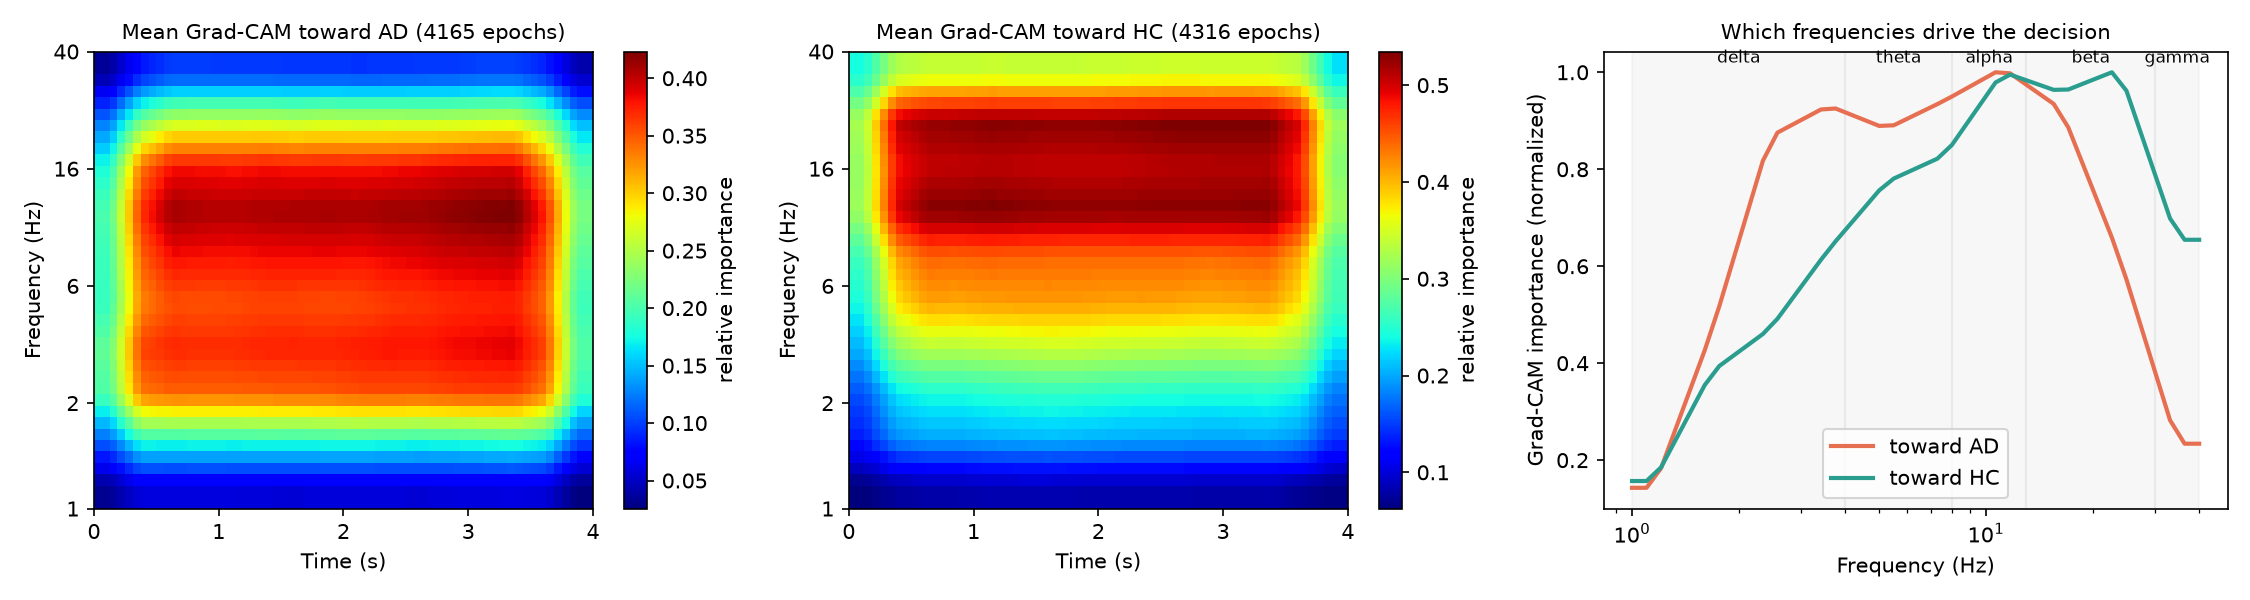
\includegraphics[width=0.9\textwidth]{cnn_gradcam.png}
\caption{Grad-CAM of the final CNN: mean maps toward AD and HC, and frequency profiles.}
\label{fig:gradcam}
\end{figure*}

\begin{figure}[t]
\centering
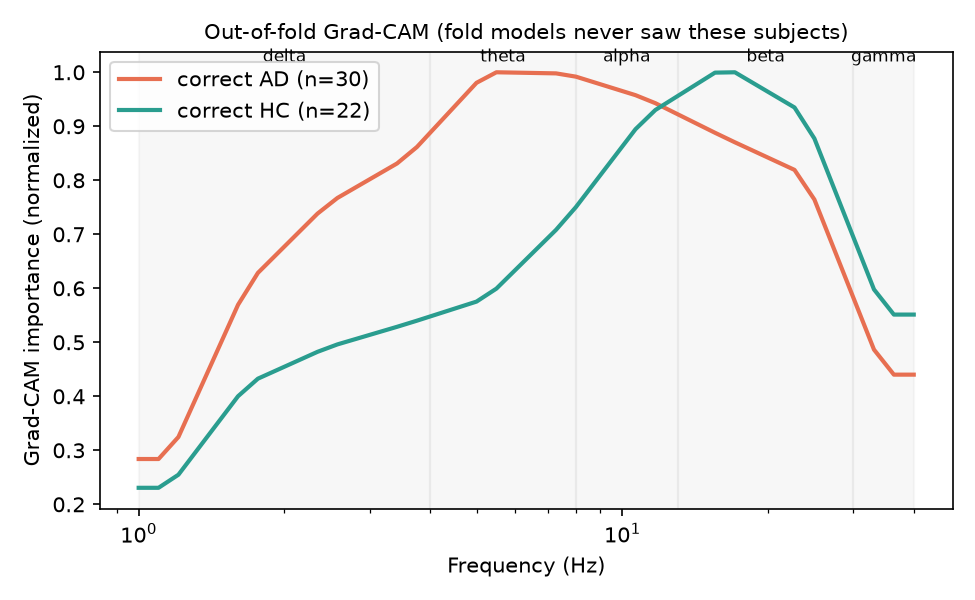
\includegraphics[width=0.85\columnwidth]{cnn_gradcam_oof.png}
\caption{Out-of-fold Grad-CAM frequency profiles for correctly classified AD and HC subjects.}
\label{fig:gcoof}
\end{figure}

\subsection{Discussion}
\emph{Brain age as deviation, not acceleration.} The brain-age framework assumes that disease moves a brain along the healthy-aging trajectory. For resting-state EEG spectra in AD, our data contradict this. AD and normal aging share alpha slowing, but they diverge on beta power, absolute slow-wave power and the aperiodic component. This agrees with electrophysiological accounts that separate pathological slowing from normal aging~\cite{babiloni2020}. A model of healthy aging places AD EEG off its trajectory, and the resulting gap is negative. The reversal was AD-specific (absent in FTD) and survived changes of model, features, harmonization, ICA, training-set size and age coverage (20--80 years). Healthy older adults from an independent laboratory did not show it. This argues against an artifact of one pipeline or site. The contrast with elevated sleep-EEG brain age in dementia~\cite{sun2019} may reflect differences in brain state, features and cohorts. Practically, a negative BAG in AD should not be dismissed as model failure: its magnitude still separates groups. It is better described as a normative deviation, and multivariate normative models of EEG spectra are a natural next step.

\emph{Classification.} The CNN exceeded the AUC~$\geq0.75$ target and was statistically indistinguishable from spectral baselines and EEGNet. This is common for small EEG cohorts, where differences of a few AUC points cannot be resolved~\cite{varoquaux2018}. The CNN's added value is end-to-end learning with time--frequency explanations that are stable out-of-fold and agree with known AD physiology. The ablations indicate that cheaper montages and shorter recordings are viable for screening.

\emph{Clinical perspective.} The system produces, per subject, a brain age, a gap relative to healthy references, a probability, and plain-language reasons such as a slowed alpha peak or increased theta share. This is useful for transparency in decision support. It is not a diagnostic device, and its error rate (about one in five for the CNN) precludes stand-alone clinical use.

% =====================================================================
\section{Conclusion and Contribution}
Under strictly subject-independent evaluation on public data, this work contributes the following:

\emph{1) A normative-deviation reading of EEG brain age in AD.} A brain-age model trained only on healthy adults found AD EEG \emph{younger}, not older ($d=\bagD{}$, 95\% CI \bagDci{}). The effect is AD-specific, robust across \nStable{} stable configurations, preprocessing, training-set size and age coverage, absent in healthy older adults from an independent site, and explained by spectral features that change in opposite directions in aging and AD.

\emph{2) An explainable scalogram CNN} with AUC \cnnAUC{} and accuracy \cnnAcc{}, benchmarked honestly against four baselines on identical folds, with ablations, a three-class extension and Grad-CAM explanations validated out-of-fold.

\emph{3) Evidence on combining the modules.} The brain-age gap adds interpretability, not accuracy, and both are delivered through an open application that produces per-subject reports.

\emph{Limitations.} The clinical cohort is small ($n=65$ for AD vs.\ HC), so confidence intervals are wide. External validation covered healthy adults only; an independent AD cohort is pending. Within the 55--80-year external cohort, predicted age did not track chronological age, so the model resolves age across the lifespan but not finely within older adults. The healthy and clinical cohorts used different amplifiers. ICA was not part of the main pipeline. BAG did not track MMSE. LEMON ages are binned. No MCI subjects were available.

\emph{Future work.} Planned work includes external validation on independent clinical cohorts with AD and MCI (e.g., CAUEEG, BrainLat), normative modeling of EEG spectra and connectivity across the lifespan, longitudinal prediction of progression, and prospective evaluation with low-density, short recordings.

% =====================================================================
\section*{Data and Code Availability}
All datasets are public: OpenNeuro ds004504 and ds005385, and MPI-LEMON. Code, trained models, all results and the scripts that generate every number, table and figure in this paper are available in the project repository.

\section*{Ethics Statement}
This study used only publicly available, de-identified data collected by the original investigators under their ethics approvals. No new data were collected.

\section*{Declaration of Generative AI Use}
During the preparation of this work the authors used Claude (Anthropic), an AI assistant, to help write and debug the analysis code and to draft and edit the manuscript text. The authors defined the research question and study design, reviewed and verified all code, analyses and results, checked every reference against bibliographic databases, and take full responsibility for the content of this publication.

\section*{Author Contributions}
All authors contributed equally to conceptualization, methodology, software, validation, formal analysis, investigation, data curation, visualization, and writing (original draft, review and editing). All authors read and approved the final manuscript.

\section*{Acknowledgment}
The authors thank Prof.~Manasa, Department of Computer Science and Engineering, B.\,M.\,S. College of Engineering, for her guidance and supervision. We thank the investigators of the OpenNeuro ds004504, ds005385 (Dortmund Vital Study) and MPI-LEMON datasets for making their data publicly available.

\section*{Conflict of Interest}
The authors declare no conflict of interest.

\bibliographystyle{IEEEtran}
\bibliography{../refs}

\end{document}
